% This example is a LaTeX document showing how to use the lmproj class to
% write your report. The chapter headings are by no means prescriptive. Instead
% use an appropriate report structure for your project as you see fit.
% Use pdflatex and bibtex to process the file, creating a PDF file as output 
% (there is no need to use dvips when using pdflatex).

% Modified 

\documentclass{lmproj}
\usepackage{graphicx}
\usepackage{float}
\graphicspath{ {images/} }
\usepackage{hyperref}
\usepackage{listings}



%\usepackage[linesnumbered,ruled,vlined]{algorithm2e}
%\usepackage{algorithmicx}
\usepackage{algpseudocode}
%\usepackage{algorithmic}
\usepackage{float}
\newfloat{algorithm}{tp}{toa}

\lstset{frame=tb,
	language=bash,
	aboveskip=3mm,
	belowskip=3mm,
	columns=flexible,
	basicstyle={\small\ttfamily},
	breaklines=true,
	breakatwhitespace=true,
	numbersep=5pt,
	xleftmargin=\parindent,
	numbers = left,
	framexleftmargin=10mm,
	frame=none,
	keywordstyle=\bfseries\color{blue},
	identifierstyle=\bfseries,
	numberstyle=\color[RGB]{0,192,192},
	commentstyle=\it\color[RGB]{0,96,96},
	stringstyle=\rmfamily\slshape\color[RGB]{128,0,0},
	showstringspaces=false
}



\begin{document}
\title{Bridging the gap between offline and online learning}
\author{Avgerinos Fotios \\
        Dunlop Fraser \\
        Constambeys Timotheos \\
        Zoulis Nickolas}
\date{18 December 2015}
\maketitle
\begin{abstract}

The abstract goes here

\end{abstract}
\educationalconsent
\tableofcontents
%==============================================================================
\chapter{Introduction}
\label{intro}

\section{Motivation}
\label{intro}

Over the last decade the area of data storage, manipulation and analysis has rapidly evolved as the previous techniques and infrastructures struggled to cope with the continuous data growth and demand rate. Algorithms and systems that used to perform well, could not handle the data explosion. Companies such as Yahoo and Google realized Moore's Law is not coming to their rescue anymore and started investing on research of developing systems that could scale linearly, instead of vertically, as data volume was increasing. 

The dawn of Big Data era was marked by the development of software infrastructures that could run on commodity hardware and exploit redundancy in order to provide availability and fault tolerance. Their workflow was targeting to partition the job to numerous physical nodes in order to decrease the total computation time. These systems can be characterized as (offline) batch processing, because they compute over batches of data and do not have the requirement to respond in realtime. Many such systems may require multiple chained passes over the data in order to provide a result.

With the advancement to Web 2.0 and the rise of social networks as well as the notion of the Internet of Things (machines equipped with sensors, transferring data at an arbitrary rate) altered the existing game rules. The need was for quick response to incoming data, without having to keep track of them or perform any asynchronous analysis over them. That said, many systems started to appear that could handle the input streaming and perform online, instead of offline learning techniques. 

\section{Problem Definition}
\label{intro}

A lot of research on both offline and online systems has been made over the last years, resulting to the recording of successful commercial usage in numerous use cases. Individually speaking, batch systems can provide offline query computation, whereas streaming systems can provide online query computation. The first ones may take a lot of time to respond, but they take into account the whole picture and can recover in case of corrupted or noisy data without losing any information, as they could simply restart computations. The latter ones, while can provide low latency answers in realtime, follow the trend of input data, which is desirable if this is the use case, if any errors occur, they cannot just simply restart without losing information from their latest safepoint to the time the error was spotted.

So what if we wanted a robust system that could provide answers as soon as possible and an always-on experience, without compromising quality? A need for a hybrid emerges, and it was Nathan Marz who first came up with the term Lambda Architecture, which describes an architecture resilient to faults, while still remaining highly available from the perspective of a client. Lambda Architecture is comprised of three basic components, the Batch, the Speed and the Serving layers. Batch layer is responsible for computing query views asynchronously over batch of data. Stream is responsible for handling the most recent data input to the system and provide answers on-the-fly by maintaining an online learning model. Last but not least, the Serving layer is responsible for indexing the views of both the other layers so they can be queried in a low latency, ad-hoc way.

The problem that arises is how the views of Batch and Stream can be merged and in what way. Who should be trusted more, what kind of methods should be used for the aggregation and how applicable would one method be in a different use case scenario are only some of the research questions that naturally arise. 

\section{Contributions}
\label{intro}

Out contribution is to investigate the trade-offs of low latency responses over quality when applying machine learning algorithms over Lambda Architecture. We implemented a proof-of-concept system that follows this design and experimented with a well-known unsupervised learning clustering algorithm, K-Means. 


%==============================================================================
\chapter{Related Work}
\label{relatedwork}

\section{Theoritical Background on K-Means}
\label{relatedwork}

\section{Batch Processing}
\label{relatedwork}

\section{Stream Processing}
\label{relatedwork}

Stream Processing uses a computing science class of algorithms (streaming algorithms) for processing streams of input data. Stream Processing assumes an infinite stream of data injected into the system at periodic time intervals. Due to the large amount of input data, stream processing algorithms have a limited processing time in each input.  The stream algorithms produce approximate solutions to the problem by storing global statistics of the problem or by processing a fixed amount of input data using a sliding window method.
A distributed system allows better performance and scalability. In addition, fault tolerance provides better system reliability and maintenance. Stream processing systems available today which are fault tolerant and distributed are:

\begin{enumerate}
	\item Apache Storm is an open source project available at Apache Software Foundation. The project is in active development and it’s most up-to-date stable version is 0.9.5 in June 2015. It was originally created by Nathan Marz using the Clojure programming language and acquired by Twitter which made it open source. 
	\item Apache Spark is an open source project available at Apache Software Foundation. The most recent version is v1.5.2 released in November 2015. Apache Spark improves the performance of Apache Hadoop using a distributed memory-based architecture. Apache Sark is based on the Map Reduce programming model. However it enables applications written for batch processing to work on stream processing by grouping data into mini-batches.
	\item Apache Samza is an open source project available at Apache Software Foundation. According to Apache Documentation (http://samza.apache.org/) it is similar to the Apache Storm project. It is distributed, fault tolerant and has sub-second latency because of the Apache Kafka for messaging passing, although it is not as popular as Storm and it is in an early development.
\end{enumerate}

The differences between Spark and Storm stream processing framework are:

\begin{enumerate}
	\item Processing Time: Storm can achieve sub-second latency because each tuple is transmitted independently of the others immediately to the system. In contrast Apache Spark groups tuples in mini-bathes which delays the transmission in the order of seconds.
	\item Fault Tolerant. Storm guarantees at least one delivery and not just one. For example if the process dies after processing the tuple and before acknowledging it, then the tuple will be resent and processed twice. Spark Streaming is better with the guarantee that each event is processed exactly once.  
\end{enumerate}

\section{Lambda Architecture}
\label{relatedwork}


%==============================================================================
\chapter{Our system - Thunderstorm}
\label{systemdescr}

\section{Overall Design}
\label{systemdescr}

For our project's purposes we have chosen to use the below systems for each component of Lambda Architecture:

\begin{itemize}
	\item Serving layer with Apache HBase
	\item Batch layer with Apache Spark
	\item Stream layer with Apache Storm
\end{itemize}

\begin{figure}[h]
\centering
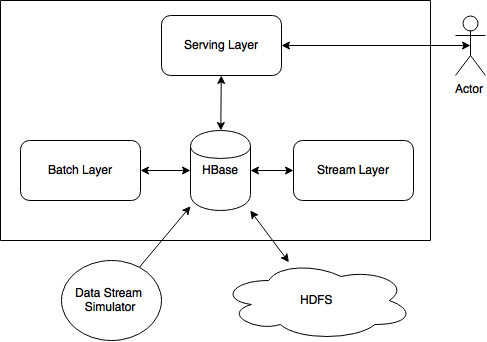
\includegraphics[width=10cm, height=8cm]{system}
\caption{An abstract picture of how our system is formulated}
\end{figure}


\section{Serving Layer}
\label{systemdescr}


Serving layer is the front-end of our system, responsible for a wide range of tasks. The interface with the external users is based on a shell-like environment. The complete command manual of the serving layer's shell is described in the Appendix section. Our system supports both plain K-Means and constrained queries (in current version maximum of 1 constraint expression). Behind the front stage, serving is responsible for storing and indexing the queries as well as the answers (views) that both batch and stream layer provide. For this task we use Apache HBase.

\subsection{Overview of HBase}
HBase is the open-source clone of Google's Bigtable, a highly scalable fault-tolerant database that can scale horizontally, maximizing random read and write throughput. Its design classifies it to the column-family NoSQL databases and can be conceived as a multidimensional sorted map. The relying data storage system is HDFS.

The basic structure is the HTable, where each row can contain multiple columns and column families, with the restriction that the latter have to be declared at the time the table is instantiated. A column family is used to group together columns with similar access patterns to optimize read and write throughput. Each row is uniquely identified by the triple $row key-column key-timestamp$ and each value in the row is an uninterpreted array of bytes (only table's and column families' names have to be appropriate for a system's filepath names). Automatic sorting is performed based on the rowkey, so clients can control their data locality via selecting custom rowkey format. More than one version of data is maintained using different timestamp label and by default the system returns the most recent one.

When an HTable reaches a threshold of rows stored in it, it partitions itself and each partition is assigned to an HRegionServer. An HRegionServer is responsible for one or more rowkey ranges. There is always on HMaster that is responsible for region assignment and create/delete table operations. HMaster uses Zookeeper to maintain which servers are live and available, which uses consensus to do so.

\subsection{Why HBase}

The basic reason we have inclined to HBase is its CAP theorem principles. CAP theorem states that distributed systems have to compromise on each of the following (Consistency, Availability, Partitioning). For our use case we wanted a distributed database that should be able to support consistent writes and reads, as well as low latency scans and sequential reads. Two big players that align with the above features, and also are well tested and documented, seem to be HBase and Cassandra. The first one opts for Consistency and Partitioning, where as the latter one opts for Availability and Partitioning. For the case of Cassandra, it is possible to tune the level of consistency by using different modes (all, one, quorum). HBase is well integrated with Hadoop, so has the advantage of playing well with MapReduce, and for a future time this could be ideal for us while having to deal with raw dataset and machine learning algorithms applied to them. Both provide easy to use Java API which was in line with our system's language support. Weighting the above factors, and since HBase offered more straightforward handling of consistency than Cassandra, we have made the design decision to use HBase as our Serving layer's major component. 


\subsection{Implementation of Serving layer}


\subsubsection{HBase schema}
Our HBase schema consists of 5 HTables:

\begin{enumerate}
	\item Raw data: Stores the whole dataset, each row consisting a data point under a single column family, using a column foreach dimension. Rowkey is a float monotonically incrementing counter.
	\item Queries: Stores the users' queries. Rowkey is a float monotonically incrementing counter. The first row of this table is specially used to hold the maximum counter of the rows, which is used from both layers to locate the new incoming queries. The user's K-Means query is stored in two columns, a column for an Integer array of bytes containing the K cluster number and a String array of bytes in an other column (both columns under the same column faimily).
	\item Batch views: Stores the results of the queries processed by the batch layer as views. Rowkey is a float number indicating the query in Queries table that corresponds to this view. There is one column family that contains as many columns as the query requires. As a column identifier is use a string prefix along with an Integer monotonically increasing counter.
	\item Stream views: Stores the results of the queries processed by the stream layer as views. The same design applies as in Batch views table.
	\item Messages: Stores an Integer counter under a single column family and column. This counter is updated by Batch layer at the end of each round of query computation and is used by Stream layer in order to detect when a computation round has finished and should synchronize its views with Batch layer's views as a feeding source. 
\end{enumerate}

\subsubsection{Event messaging simulation}
The serving layer is responsible for the coordination of both Batch and Stream layer. There is a need for simulating the queue of events happening in our system, and whereas there are a variety of messaging systems out there appropriate for this task such as Kafka and RabbitMQ, we have made the design decision to follow the simplest approach possible to minimize complexity, and simulate the queue via HBase. Serving layer puts queries in HBase and then starts polling for result views, and both Batch and Stream layers periodically poll HBase in order to detect any incoming query and start computation.

\section{Batch Layer}
\label{systemdescr}

\section{Streaming Layer}
\label{systemdescr}

\subsection{Overview of Storm}

Apache Storm is an open source project designed to handle online data. Storm can process continues streams of data on-the-fly.  Its topology makes it extremely flexible to adapt to any scenario. It provides fault- tolerant guarantees in case server nodes fail. Storm internally uses the Apache ZooKeeper open source project which is a fault tolerant way to pass messages between nodes. Additional data processing guarantees are provided by explicitly declaring processed Tuples using acknowledgement messages. Storm has the following types of nodes in a cluster:

\begin{itemize}
	\item The master node. The master mode is called Nimbus daemon. According to the Storm documentation by apache [1], the nimbus node is important but the system does not die when then nimbus fails. This node can be used for monitoring the system and deploying the cluster code to the worker nodes. Since Hadoop also uses the ZooKeeper project the master node is similar to the JobTracker.
	\item Supervisors. Supervisor nodes are part of the Zookeeper Project (Apache ZooKeeper) which provides coordination between the master node and the worker nodes. The supervisor nodes can restart the worker nodes even if the master node is not responding but they cannot reassign workers to different nodes in case the worker is dead.
	\item •	Worker nodes. The worker nodes are where the processing of the data takes place. The worker daemon listens for requests from the supervisor nodes and starts and stops the worker processes as necessary.
	
\end{itemize}

A Storm Topology is layout of the system’s dataflow. The topology runs forever since Stop concept is based on continues steams of data.  More specifically the Storm Topology is the data flow network constructed from Spouts and Bolts. Spouts and Bolts are the two types of worker nodes available and they communicate using streams and tuples. 

\begin{itemize}
	\item Tuple. A  Tuple contains fields which are declared in the declaration of the stream. Each field can contain the java native types and custom types which implement the java Serializable Interface
	\item Stream. A stream can contain multiple tuples emitted by bolts or spouts. Bolts and Spouts can declare multiple streams and assign in each stream a unique id. In case no id is specified, Storm gives the stream the ‘default’  id 
	\item Spouts. A Spout is a source of streams in a Topology. Spouts can emit tuples in the topology together with a unique message id. When a tuple is received then the sender must acknowledge the tuple. If it fails to acknowledge then the fail method in the spout class will be called after the timeout expires. An important observation is that the Storm Topology does not guarantee reliable delivery by automatically resending the tuple. However the spout can be aware that either the tuple has been successfully processed or failed.
	\item Bolts. The bolt is the core component of the Storm’s Topology. Bolts are the processing nodes where different types of operations can be performed such as filtering, functions, aggregations, joins etc. Bolts can receive streams from spouts or other bolts and outputs streams to other bolts.
\end{itemize}

Storm allows multiple entities running within a cluster node based on the following concept:

\begin{itemize}
	\item Worker processes. Machines in the Topology can run multiple worker processes 
	\item Executors (threads). A worker process can have multiple executors (threads) for executing worker’s tasks.
	\item Tasks. A task can be a Spout or a Bolt
\end{itemize}

Example of a Topology from the Storm Website

\begin{tabbing}
	\hspace*{2cm}\=\hspace*{1cm}\= \kill
	\> 1. \> Config conf = new Config(); \\
	\>    \> // use two worker processes  \\
	\> 2. \> conf.setNumWorkers(2); \\
	\>    \> // set parallelism hint to 2 \\
	\> 3. \> topologyBuilder.setSpout("blue-spout", new BlueSpout(), 2); \\
	\> 4. \> topologyBuilder.setBolt("green-bolt", new GreenBolt(), 2) \\
	\>    \>  \hspace*{2cm} .setNumTasks(4) \\
	\>    \>  \hspace*{2cm} .shuffleGrouping("blue-spout"); \\
	\> 5. \> topologyBuilder.setBolt("yellow-bolt", new YellowBolt(), 6) \\
	\>    \>  \hspace*{2cm} .shuffleGrouping("green-bolt"); \\
	\> 6. \> StormSubmitter.submitTopology(  "mytopology", conf , \\
	\>    \>  \hspace*{2cm} topologyBuilder.createTopology() \\
	\>    \>  \hspace*{2cm} ); \\
		
\end{tabbing}

The Topology constructed from the code above creates a Topology example with a Blue Spout, a Green and a Yellow Bolt. Firstly the $conf.setNumWorkers(2);$ \space [2] creates two worker processes that are distributed on two different machines on the network

The $setSpout("blue-spout", new BlueSpout(), 2);$ \space [3] creates 2 Blue Spouts each with its own thread that run on each worker.

The $setBolt("green-bolt", new GreenBolt(), 2)$ \space [4] differs from the blue because the number of tasks was set to 4. As a consequence the green bolt will create 2 threads (one on each worker) and each thread will run 2 green bolts.

The $setBolt("yellow-bolt", new YellowBolt(), 6)$ \space [5] is similar to the blue spout because each bolt will run in its own thread. Since the worker processes are only 2, 3 bolts will run on the same process (worker). 

\subsection{Implementation of Streaming Layer}

The streaming layer implemented can handle many online k-means algorithms and can update their state by reading continues streams of data from a local file or a database (HBase). The data are propagated through the Storm Topology and are processed by the bolt nodes. The k-means algorithms can have filtering rules that filter data which do not meet the specified conditions. At specified time intervals the results are displayed to the user or written in the database. The Storm topology consists of the following entities:


\begin{itemize}
	\item Signals Spout. The signal spout is responsible for generating signal requests. The print signal request outputs the current state of the kmeans algorithms to the Output Bolt. The clear signal request resets or clears the state of the k-means algorithms to the initial state or to state available by batch layer.
	\item Commands Spout. The commands spout is responsible for reading the queries and the filters from the HBase and submit the query in the topology. A new instance of KMeansOnline class is created which implements the java serializable interface in order to be able to be used as a custom tuple. If all the queries from the HBase table have been read, a run signal is broadcasted to the input spouts responsible for reading the points. This ensures that the processing of the input data will not start before the initialization of all the k-means algorithms. 
	\item Points-reader Bolt. The Points-reader Bolt reads the given input file after a commands spout signal and emits each line to the points-processor bolt.
	\item Points-processor Bolt. The Points-processor Bolt receives each line of the file and converts it into a Point class.  The Points class is a custom class defined in the bridge project.
	\item Points-Reader-HBase. The Points-Reader-HBase bolt is responsible for continuously polling the HBase database for new points and emits them to the system. At the beginning of the project because no database implementation was available, the previous two modules were used. Later these two were replaced by this module. 
	\item Bolt-Processor. The bolt processor is responsible for storing the k-means algorithms and updates them based on new points.  Any number of bolt processor modules can be configured in the Storm Topology, each responsible for a set of k-means algorithms. However the input data must be distributed to all Bolt-Processor modules. For the demonstration of the system the Bolt-Processor modules was set to 2.
	\item Output-bolt. The output bolt was created in order to have a centralized point were results will be sent. The output bolt can displays the results of the k-means algorithms to the user or updates the database tables. Only one output bolt is available in the Topology in order to avoid concurrency related issues.
	
\end{itemize}

\begin{figure}[H]
	\centering	
	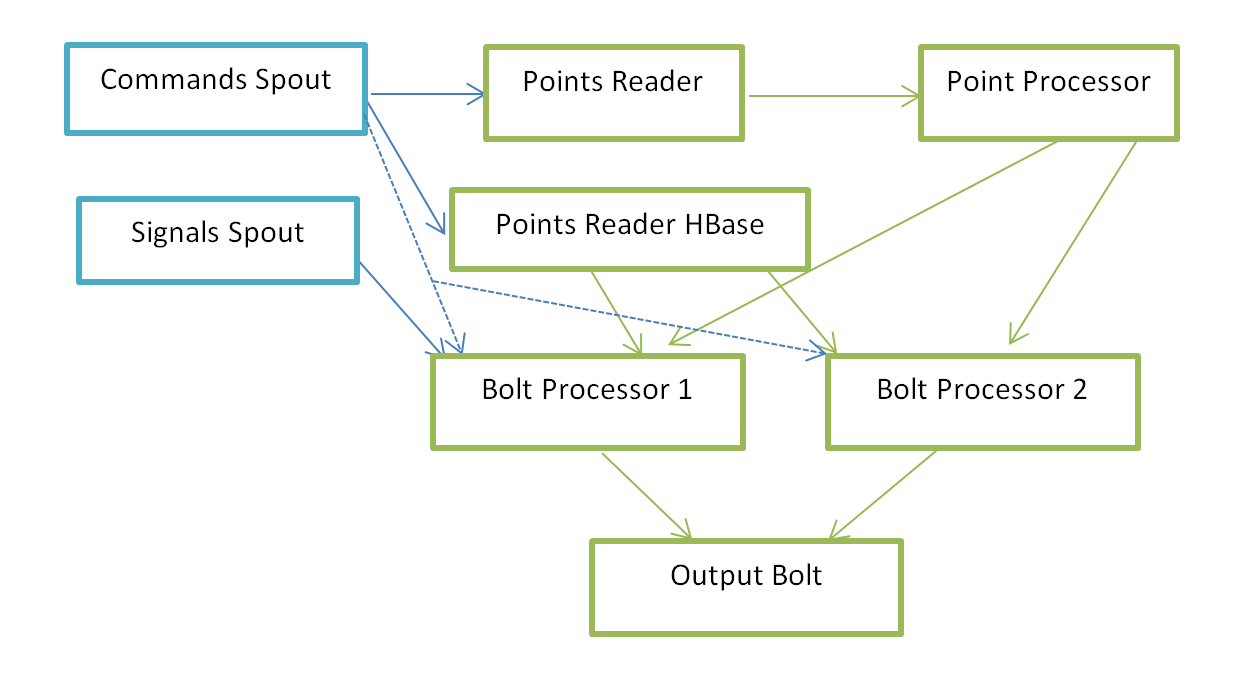
\includegraphics[scale=0.5]{topology}
	\caption{Streaming layer Topology. The blue boxes are spouts and the green boxes are bolts. Links show the flow of tuples between nodes. The dotted blue lines from the commands spout indicate that k-mean tuples are distributed in each node.}
\end{figure}


\subsection{K-Means Algorithm}

The k-means algorithm is a clustering algorithm which given a sequence of measurements $x_{1}$, $x_{2}$, $x_{n}$ , it calculates k representative point $\mu_{1}$, $\mu_{2}$, $\mu_{k}$ which minimize the square of absolute distances of each measurement to the closest point $\mu_{i}$.

\begin{figure}[hp]
	\centering	
	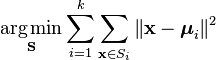
\includegraphics[scale=1.5]{kmeans}
	\caption{Source: Wikipedia}
\end{figure}

The online k-means is based on the offline k-means algorithm but it does only one iteration. The steps of online k-means algorithm are:

\begin{itemize}
	\item Initialize $\mu_{1}$, $\mu_{2}$, $\mu_{k}$  using the first k points of the stream
	\item Set the counters $c_{1}$, $c_{2}$, $c_{k}$  to 1
	\item Repeat forever
	\begin{itemize}
	\item Read the next input point $x_{i}$
	\item Calculate the Euclidian distance between each cluster center $\mu_{1}$, $\mu_{2}$, $\mu_{k}$
	\item Find the minimum distance
	\item Increment counter $c_{i}$
	\item Update cluster center using the formula
	\[ \mu_{i} = \mu_{i} + \frac{1}{c_{i}} * (x_{i} - \mu_{i} )\]
	\item Or using a fixed constant $c$
	\[ \mu_{i} = \mu_{i} + c * (x_{i} - \mu_{i} )\]
	\end{itemize}
\end{itemize}

The implementation of the online k-means algorithm is done by the K-Means Online class. The k-means online class can be constructed using its constructor and giving as parameters the query unique id and the number of clusters (k). It then initializes two arrays of size k, one for the counters of each cluster and another one an array of Point types. The Point class is a created to hold multi-dimensional points and perform vector operations such as addition, multiplication, division, distance etc. 

\subsection{K-Means Improvement}

The online k-means algorithm updates its status with each new input data. As a result, it is highly dependent on the input data. The fist k points are read from the input and are assigned into cluster centers. These points must be evenly distributed into the space in order to have better distribution of clusters in the space. To avoid bad selection of initial points, more initial points can be selected resulting in a larger number of clusters. At the end of the algorithm the closest clusters can be merged producing the desired number of clusters.

The CONSTANT variable in the K-Means-Online class is multiplied with the requested number of clusters, for example k. The algorithm stores k times constant clusters. When the results of the clustering are requested, the k times constant clusters are reduced to k by merging the closed clusters together.

\subsection{Points Filtering}

The k-means algorithms can have multiple filters and n dimensional input data. Input data that do not satisfy the filters are ignored. The k-means online class implements an add method which accepts a Data-Filter class. The Data-Filter class internally relies on the JavaScript evaluator class to evaluate mathematical expressions. At runtime the symbolic notation of the data is replaced by the real data and the javascript evaluates the expression. A filter can be of the form:

 \begin{itemize}
 	\item
 	\begin{minipage}[t]{0.3\linewidth}
 		$x0 = 10$
 	\end{minipage}%
 	\begin{minipage}{.7\linewidth}
		// The first component of the input must be 10
 	\end{minipage}
 
 
 	\item
 	\begin{minipage}[t]{0.3\linewidth}
	 	$x0 + x1 + x2 > 10$
 	\end{minipage}%
 	\begin{minipage}{.7\linewidth}
 		// The first, second and third components of the input must be greater than 10
 	\end{minipage}
 \end{itemize}


\section{Interfacing between the layers}

All the layers of the system use the HBase database to synchronize their communication. This guarantees that the communicating channels are fault tolerant. The bridge module provides the classes for reading and writing data to HBase. The communication between the HBase and the real-time layer is listed below:

\begin{itemize}
	\item Commands Spout. The commands spout monitors the queries table in HBase database for new queries.  New queries can start from scratch or use a seed from the batch layer. 
	\item Bolt Output. This bolt updates the HBase database with the new real time results
	\item Signals Spout. The signal spout monitors the HBase database for updates in batch layer data. If new batch results are found in the database, the signal spout informs the Bolts to reinitialize their k-means algorithms 
\end{itemize}

The synchronization of the online and offline k-means algorithm enables the online k-means to update its knowledge from the batch layer. Because the offline algorithm produces more reliable results than the online, the online algorithm uses the most up-to-date offline knowledge and updates it as new data enter the system. However, the offline k-means algorithm takes a lot of time to complete and the new data that enter the system while the algorithm is running are ignored. In order to avoid this, when the offline algorithm starts a new computation round, the online algorithm creates a new copy of the current queries which do not print any results. When the computation round end, the old queries are replaced by the new queries combining their results with the offline algorithm. The following diagram shows how these events happen in time. The yellow boxes represent the batch’s layer computation round. The green boxes represent the active queries, i.e. queries enabled for print output and the blur boxes represent the new hidden queries 

\begin{figure}[H]
	\centering	
	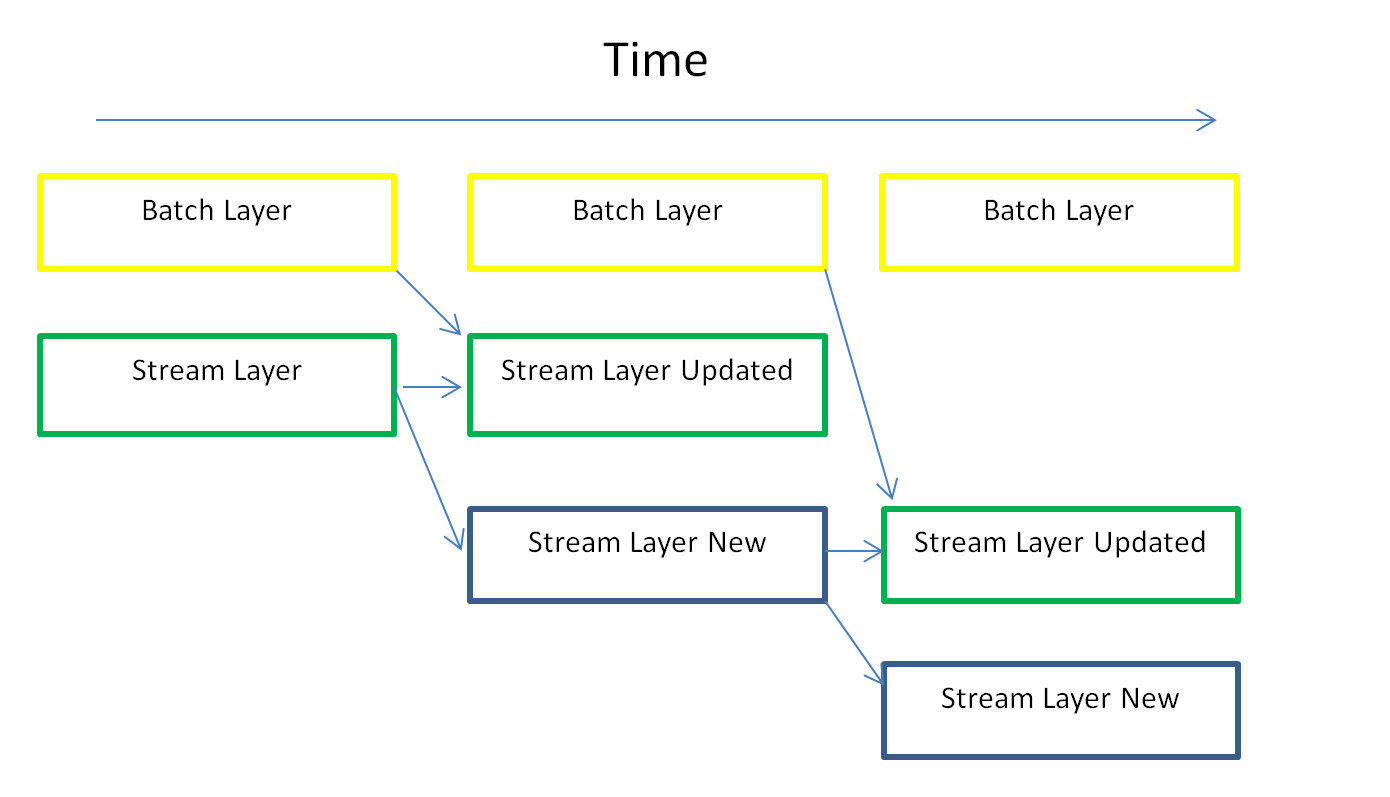
\includegraphics[scale=0.4]{synchronization}
	\caption{Synchronization between the online and offline layers.}
\end{figure}

\section{Data stream simulation}
\label{systemdescr}
We use a separate module to simulate the data stream in our system. It can be configured to periodically read ranges of data from a raw file and extract specific columns (dimensions) and put it in HBase. 



%==============================================================================
\chapter{Offline/Online K-Means}
\label{kmeans}

\section{Theoritical Solution outline}
\label{kmeans}

\section{Baseline Solution}
\label{kmeans}

In order to be able to answer queries as soon as possible we came up with the an algorithm that is composed of a sequence of checks and respective actions. We will describe this algorithm with both use case pseudocode and a flowchart.


\bigskip


	\begin{algorithm}[H]
		\caption{KMeans Solution}\label{kmeanssolution}
		\begin{algorithmic}[1]
			\Procedure{KMeans}{$Query$ $K$}
			\Require Stream is fed views from Batch
			\Require $K<<K'$
			
			\If {Query K is new}
				\State Put it in HBase
				\State Batch and Stream start computing views
			\Else 
				\If {Stream has a view}
					\State \Return view
				\Else 
					\State Do a $K-out-of-K'$ local KMeans
					\State \Return view
				\EndIf
			\EndIf			
			
			\EndProcedure
		\end{algorithmic}
	\end{algorithm}



\begin{figure}[H]
	\centering	
	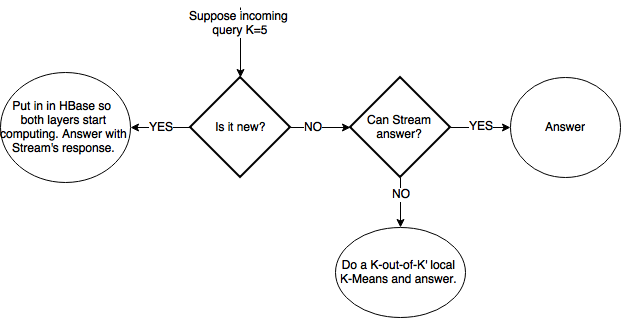
\includegraphics[scale=0.5]{usecase}
	\caption{Solution flowchart}
\end{figure}


\section{Fusion Scheme}
\label{kmeans}




%==============================================================================
\chapter{Evaluation}
\label{evaluation}

\section{Setup}
\label{evaluation}

\subsection{Hardware Specifications}
Our experiments were conducted in a Virtual Machine with the below specifications:
\begin{itemize}
	\item 1.6 GHz dual core Intel Core i5
	\item 2GB RAM
\end{itemize}

\subsection{Software Specifications}
Our experiments were conducted using the below software:
\begin{itemize}
	\item hadoop-2.6.2
	\item hbase-0.98.15-hadoop2
	\item spark-mllib-2.10
	\item storm-core-0.9.5
	\item unix operating system
	\item java 1.7
	\item maven
\end{itemize}

\subsection{Dataset Normalization}
Our dataset consists of 100.000 rows of 8-dimensional data (gas leak concentrations). We have preprocessed the dataset by normalizing it using Standard Score normalization. The standard score of a raw score is $x$ :

\begin{figure}[h]
	\centering
	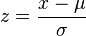
\includegraphics{standard_score}
	\caption{From Wikipedia}
\end{figure}

where:
\begin{itemize}
	\item $\mu$ is the mean of the population
	\item $\sigma$ is the standard deviation of the population.
\end{itemize}

\subsection{Silhouette Score}

\subsection{Experiment setup instructions}

Our system should be able to be deployed in any Unix operating system. We have tested it under a Debian distribution. Should someone is willing to reproduce our experiments, oughts to have at least Java 7 installed along with Maven 2. 

There is a single file in our project containing all of our configuration variables as static final Java variables ($bridge/src/main/java/hbase/Cons.java$). The project is setup this way so only one variable has to be changed in order to have the system ready for deployment, and this is $hbaseIPaddress$. We have configured Hadoop and HBase in pseudo-distributed mode, where as Spark and Storm run on stand-alone mode. A user is able to change the above configuration at will. 

After having the above requirements configured, our project can be built as follows:

\begin{itemize}
	\item Clone from github:   \url{https://github.com/nickozoulis/master_team_project} 
	\item From command line move to root directory
	\item Execute $mvn$ $clean$ $package$ 
	\item Each module will produce a jar under $/module/target/$ folder
\end{itemize}

Following example commands describe how to run the modules, all executed from the root project folder:

\begin{enumerate}
	\item data stream simulator
	\item serving layer
	\item batch layer
	\item stream layer
\end{enumerate}

\noindent Bash commands :
\begin{lstlisting}[language=bash]
$ [1] java -jar data_stream_simulator/target/data_stream_simulator-{..}-jar-with-dependencies.jar -f {filepath to normalized dataset}
\end{lstlisting}

\begin{lstlisting}[language=bash]
$ [2] java -cp serving_layer/target/serving_layer-1.0-SNAPSHOT-allinone.jar {option -f with a given queries file}
\end{lstlisting}

\begin{lstlisting}[language=bash]
$ [3] java -cp batch_layer/target/batch_layer-{..}-allinone.jar Main
\end{lstlisting}

\begin{lstlisting}[language=bash]
$ [4] java -jar realtime_layer/target/realtime_layer-{..}-jar-with-dependencies.jar
\end{lstlisting}

\section{Results}
\label{evaluation}

\section{Discussion}
\label{evaluation}


%==============================================================================
\section{Conclusions}
\label{conclusions}


%==============================================================================
\bibliographystyle{plain}
\bibliography{example}
\end{document}
